\pagestyle{empty}
\frontmatter
\begin{titlepage}
\begin{textblock*}{210mm}(0mm,0mm)
   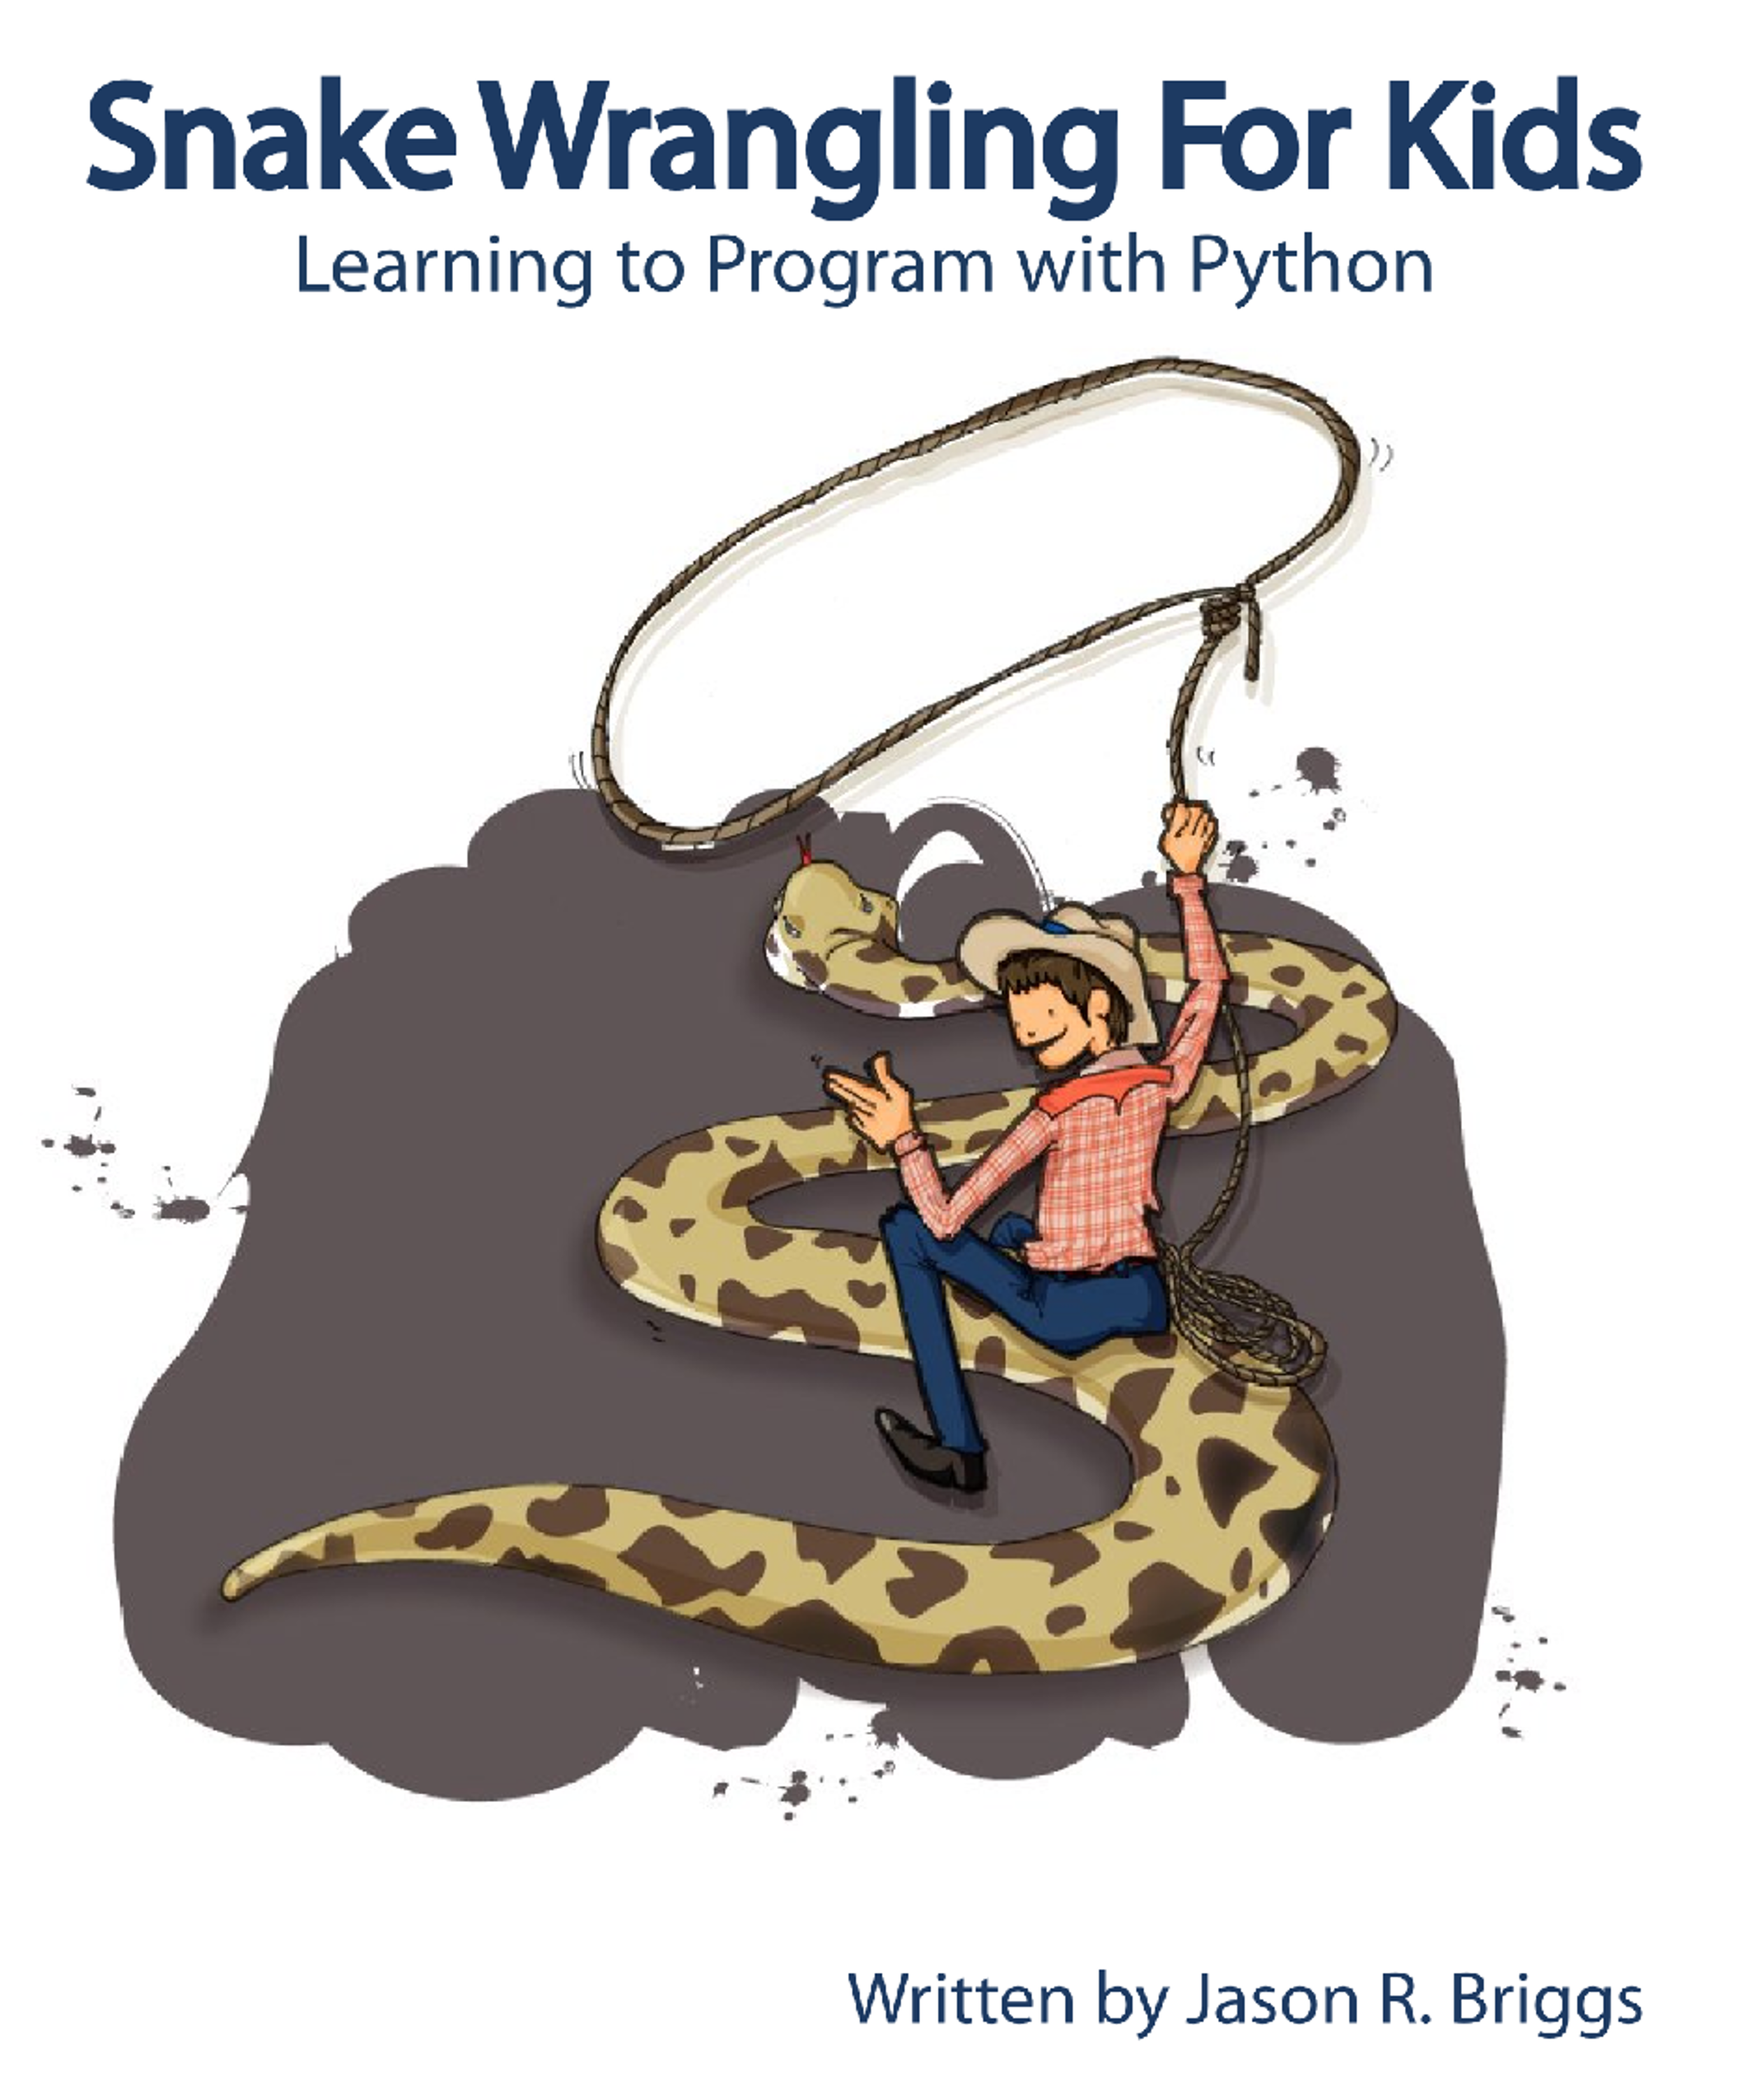
\includegraphics[width=0.9\paperwidth]{cover.eps}
\end{textblock*}
\begin{flushright}
\begin{WINDOWS}
\includegraphics[width=40mm]{windows-edition.eps} 
\end{WINDOWS}
\begin{MAC}
\includegraphics[width=40mm]{mac-edition.eps} 
\end{MAC}
\begin{LINUX}
\includegraphics[width=40mm]{linux-edition.eps} 
\end{LINUX}
\end{flushright}
\end{titlepage}

\noindent
\textsf{\emph{Snake Wrangling for Kids, Learning to Program with Python}}\\
by Jason R. Briggs\\
\\
Version 0.7.6
\\\\
Copyright \copyright 2007.\\
\\
Published by... ah, no one actually.\\
\\
Cover art and illustrations by Nuthapitol C.\\
\linebreak 
\noindent
Website:\\ \href{http://www.briggs.net.nz/log/writing/snake-wrangling-for-kids}{http://www.briggs.net.nz/log/writing/snake-wrangling-for-kids}\\ 

\noindent
Thanks To:\\
Guido van Rossum (for benevelont dictatorship of the Python language), the members of the Edu-Sig mailing list (for helpful advice and commentary), and author David Brin (the original instigator of this book).\\

\noindent
License:\\
This work is licensed under the Creative Commons Attribution-Noncommercial-Share Alike 3.0 New Zealand License. To view a copy of this license, visit\\ \href{http://creativecommons.org/licenses/by-nc-sa/3.0/nz/}{http://creativecommons.org/licenses/by-nc-sa/3.0/nz/} or send a letter to Creative Commons, 171 Second Street, Suite 300, San Francisco, California, 94105, USA.\\

\noindent
Below is a summary of the license.\\

\noindent
You are free:
\begin{itemize}
 \item \textbf{to Share} — to copy, distribute and transmit the work 
 \item \textbf{to Remix} — to adapt the work
\end{itemize}
\noindent
Under the following conditions:
\begin{description}
 \item[Attribution.] You must attribute the work in the manner specified by the author or licensor (but not in any way that suggests that they endorse you or your use of the work).
 \item[Noncommercial.] You may not use this work for commercial purposes.
 \item[Share Alike.] If you alter, transform, or build upon this work, you may distribute the resulting work only under the same or similar license to this one.
\end{description}

\noindent
For any reuse or distribution, you must make clear to others the license terms of this work.\\

\noindent
Any of the above conditions can be waived if you get permission from the copyright holder.\\

\noindent
Nothing in this license impairs or restricts the author's moral rights.\\

\mainmatter

\pagestyle{plain}

\pagenumbering{roman}
\tableofcontents